\section{Energy Demand and Supply}
At the basis of our work is the knowledge of a rapresentative, realistic demand profile, that would catch the transient of the energy deamnd throughout the year.
Given our focus on the residential sector, the overall energy demand can be seen as the sum of the heating/cooling contribution + all the other electricity consuptions for appliances and lightning.
Based on the available data we have chosen to model the system based on the distribution of energy classes.
Several semplifications will be made through the following derivation but we point out any possible improvment that could be made but was considered out of the scope of this work.

\subsection{Methodology}
We utilize energy classes to characterize residential homes based on data from the CENED database. 
In Italy, an APE (Attestato di Prestazione Energetica) is a document that certifies the energy performance of a building. 
This certification must be issued by a qualified technician and is mandatory for all buildings that are sold or rented. 
Each residential unit, corresponding to the residence of a single family, requires its own APE. 
For instance, a building with three apartments will have three separate APEs, one for each apartment.

By analyzing the APE database, we can establish correlations between energy classes and specific building characteristics, 
such as the presence of photovoltaic (PV) installations or heat pumps. 
This approach allows for the easy modification of future scenarios by adjusting the distribution of 
energy classes across the total number of buildings. 
Our objective is to determine the most relevant characteristics of each energy class and to derive 
a representative energy demand profile for each class.

From the CENED database \cite{cened2025} we extracted the information about the relevant municipalities of the region,
which we derived based on the map of primary substations from the national grid operator (GSE) \cite{gse_cabine_primarie}.
The data was also filtered to include only residential buildings, excluding commercial and industrial ones.
This was necessary given the large amount of data from the complete regional database. This way an easier to manage csv file was obtained.
Note that an API is available to access the database but it was found to be very slow and inefficient.

\subsection{Heating and Cooling Demand}
For each energy class we have taken a real example of a residential building from the region under study and computed the 
hourly thermal demand for heating and cooling thoughout the year.
This is obtained by means of a professional software (TERMOLOG) that allows for dynamic simulation of the energy system of the building.
This computation is based on the UNI EN ISO 52016 standard.
We used one reference building per energy class all with the same utlization profile, which is a simplification to be discussed later.
The output of the calculation is an hourly profile of the thermal demand for heating and cooling.

% Add one example of the houdly profile

\subsubsection{Normalization of the Data}
The data of each building had to be normilized to be rapresentative of the "average building".
To do so we used the "userful heated area" information from the CENED database.
This is the area of the building that is actually used for heating and cooling, excluding areas such as garages, attics, and basements.
We normalized the reference profiles over their area and then used the average area 
of the buildings removing the top 99 buildings since some anomalies have been encountered.
The average area ended up being $91.37 m^2$.

\begin{figure}[H]
    \centering
    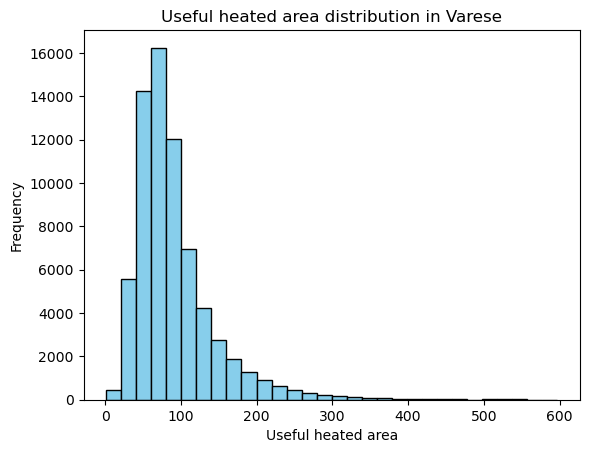
\includegraphics[width=0.8\textwidth]{figures/1_building_area_histogram.png}
    \caption{Histogram of the useful heated area of buildings.}
    \label{fig:building_area_histogram}
\end{figure}

\subsection{By class distributions}
To be able to simply simulate different scenarios we have identified characteristics of each energy class 
so that we can just modify the energy calss distribution and all the parameters needed to determine the energy demand will follow.

\subsubsection{Heat Pump distribution and Cooling Demand}
We identified the share of heat pumps per energy class.
We also determined the share of buildings that have a cooling system installed, which as of today comes up to $9.58\%$. 
This is a very low share and is to be expected as the region under investigation is quite chill during summer.

\begin{figure}[H]
    \centering
    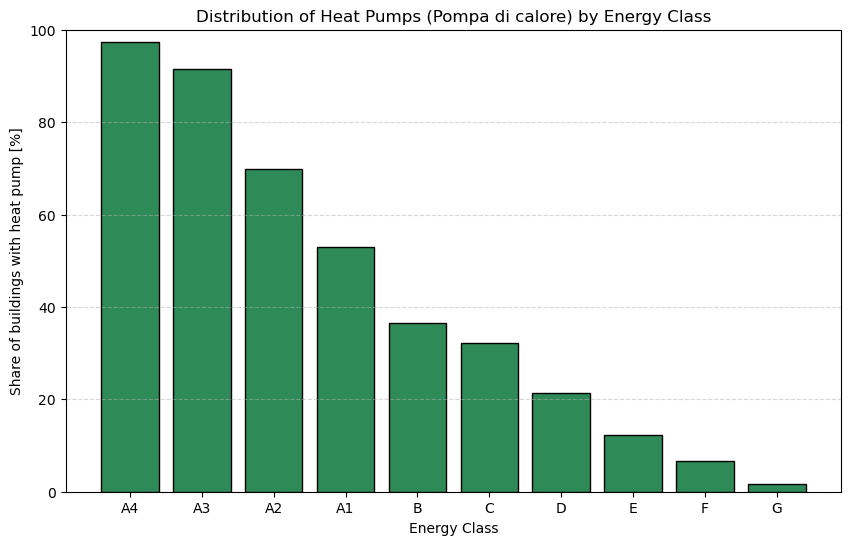
\includegraphics[width=0.8\textwidth]{figures/1_heat-pump-share.png}
    \caption{Distribution of heat pumps across energy classes.}
    \label{fig:heat_pump_distribution}
\end{figure}

\begin{lstlisting}[language=python, caption={Code to extract heat pump data from the CENED database.}, label={lst:heat_pump_query}]
    df = pd.read_csv(path, dtype=str) # Read the data
    energy_classes = ["A4", "A3", "A2", "A1", "B", "C", "D", "E", "F", "G"]
    impianto_cols = [col for col in df.columns if 'TIPO_IMPIANTO' in col]
    has_pdc = df[impianto_cols].apply(lambda row: row.str.lower().str.contains('pompa di calore', na=False).any(), axis=1)
    classe = df['CLASSE_ENERGETICA']
    total_by_class = classe.value_counts()
    pdc_by_class = classe[has_pdc].value_counts()
    total_by_class = total_by_class.reindex(energy_classes, fill_value=0)
    pdc_by_class = pdc_by_class.reindex(energy_classes, fill_value=0) # Reorder by class
    pdc_percentage = (pdc_by_class / total_by_class * 100).fillna(0) # Calculate share
\end{lstlisting}

\begin{lstlisting}[language=python, caption={Code to extract cooling system data from the CENED database.}, label={lst:cooling_share}]
    df = pd.read_csv(path, dtype=str) # Read the data
    sup_raffrescata = df['SUPERF_UTILE_RAFFRESCATA'].astype(float)
    cooling_count = len(sup_raffrescata[sup_raffrescata > 0]) # Count how many buildings have cooling
    cooling_percentage = (cooling_count / len(df)) * 100 # Percentage of buildings with cooling
\end{lstlisting}

\subsubsection{Photovoltaic distribution}
We identified the share of buildings with photovoltaic systems installed.
\begin{lstlisting}[language=python, caption={Code to extract photovoltaic data from the CENED database.}, label={lst:photovoltaic_query}]
    df = pd.read_csv(path, dtype=str) # Read the data
    has_pv = df['CONSUMI_SOLARE_FOTOVOLTAICO'].astype(float) > 0
    classe = df['CLASSE_ENERGETICA']
    total_by_class = classe.value_counts() # Total buildings per class
    pv_by_class = classe[has_pv].value_counts() # Buildings with PV per class
    pv_percentage = (pv_by_class / total_by_class * 100).fillna(0) # Calculate percentage
\end{lstlisting}

\begin{figure}[H]
    \centering
    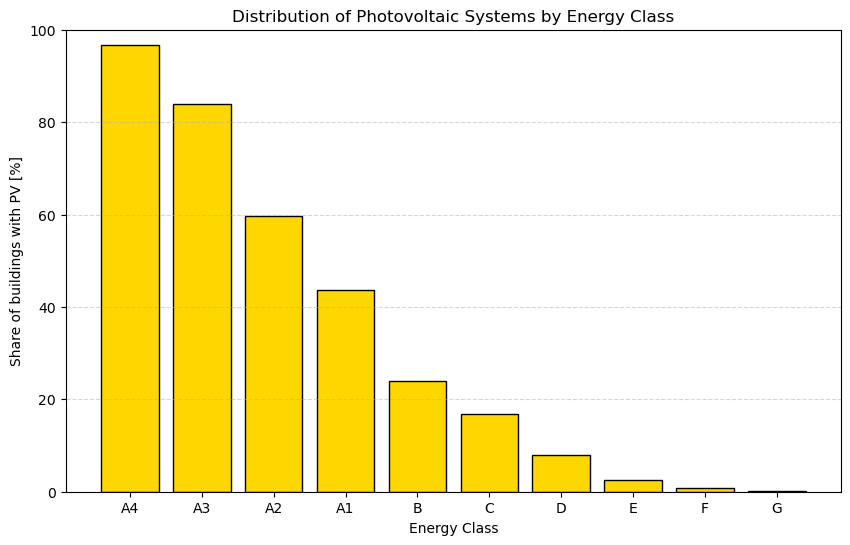
\includegraphics[width=0.8\textwidth]{figures/1_photovoltaic_distribution.png}
    \caption{Distribution of photovoltaic system sizes across energy classes.}
    \label{fig:photovoltaic_size_distribution}
\end{figure}

Another interesting information we gathered is the relative size of the photovoltaic system. 
Using data from the CENED database: Exported Electricity, Imported Electricity and In situ consumption.

\begin{equation}
    \text{SCF: Self-Consumption Factor} = 1 - \frac{\text{Import}}{\text{Export} + \text{In situ consumption}}
\end{equation}

\begin{equation}
    \text{OSF: Over-Sizing Factor} = \frac{\text{Export}}{\text{Export} + \text{In situ consumption}} - 1
\end{equation}

Mind that this data comes from the CENED 2.0 calculation system which uses a non dynamic simulation of the energy system and neglects
any storage.

\begin{table}[H]
    \centering
    \begin{tabular}{|c|c|c|}
        \hline
        \textbf{Class} & \textbf{SCF (\%)} & \textbf{OSF (\%)} \\
        \hline
        A4 & 61.51 & 3.96 \\
        A3 & 44.08 & 34.20 \\
        A2 & 31.68 & 267.82 \\
        A1 & 25.57 & 1004.33 \\
        B  & 19.29 & 947.18 \\
        C  & 15.51 & 419.08 \\
        D  & 9.16  & 102.67 \\
        E  & 3.92  & 116.66 \\
        F  & 1.15  & -68.68 \\
        G  & 0.24  & -95.72 \\
        \hline
    \end{tabular}
    \caption{SCF and OSF indicators by Energy Class.}
    \label{tab:pv_scf_osf}
\end{table}

The extreme overdimensioning on some classes can be explained with hands-on experince:
To boost the energy class of those in the middle of the scale (betwwen C and E),
it is common that contractors choose to an over sized photovoltaic system.
This effect was exagerated during the "superbonus" (2021-2023) period which required a mandatory jump of 2 energy classes to be eligible for the tax deduction.

% Still missing how we get the PV production profile, work in progress we might change the way we get the plant size.

\subsection{Convertion from thermal to primary energy demand}
The dynamic simulation outputs the thermal demand of the building. 
To estimate the primary energy needed we used average efficiencies of the heating and cooling systems.

\begin{equation}
    \dot{Q}_{\text{fossil}} = \frac{\dot{Q}_{\text{th}}}{\eta_{\text{fossil}}}
\end{equation}

\begin{equation}
    P_e = \frac{P_{\text{th, heating}}}{\text{COP}_{h}} + \frac{P_{\text{th, cooling}}}{\text{COP}_{c}}
\end{equation}

\subsection{Other Electricity Demand}
% Once we settle on the numbers report them here
Electrical demand for appliances and lighting is modeled equal for all classes.
The definition was manual, hour by hour for an average day in the following "seasons":
\begin{itemize}
    \item Winter Weekday
    \item Winter Weekend
    \item Summer Weekday
    \item Summer Weekend
    \item Winter Holiday
    \item Summer Holiday
\end{itemize}
Moreover we added an absence factor to take into account when people go on holiday massively during august.

The profile is defined by considering the following contributions:
\begin{itemize}
    \item standby and always on appliances
    \item lighting 
    \item appliances
\end{itemize}
During the summer the need for a cooling fan was added.  
Moreover we added a parameter to rapresent the share of buildings with an induction system installed.

% reference hourly profile through the year

\subsection{Total Grid Demand}
In the end we choose an energy class distribution to rapresent a future scenario.
Given that we know the reference demand-production profile of each building we can sum them up by  weighting on their supposed share to obtain the total reference demand
which is then multiplied by the number of buildings in the region to obtain the total demand.

% WIP how many buildings in the region

\subsubsection{Comparison and Tuning}
To verify our method is acceptable we compare the total demand by the data available online, in particual we compared it to the average annual deamnd,
in the residential sector for the province of Varese \cite{portaleconsumi_energia_domestica}, which happends to be $1931 kWh$ in 2023,
with a decreasing trend in the last years ($2016kWh$ in 2022 and $2119kWh$ in 2021). 

% WIP tuning the data

\subsubsection{Possible Improvments}
It is defenitly possible and could give better results if the data for each class was obtained by a set of real building from the region instead of just one.
Ideally one would use a statistically signfinicant set of buldings and vary the utilization profile as well.
Moreover, it would be beneficial to wheight the simulation data on the real energy requirments of those same buildings,
which is a much more complex task since it would require extensive data acquisition during the year. 
While this is feasible for electrical demand (most operators give to the customer a detailed bill with hourly consumption),
it is much more difficult to get the same data for fossil fuel consumption.
At last, the normalization has been done with the heated area an not with the volume (which is much more indicative of the energy requirment of a building) 
given the on-field knowledge that the volume is usually approximatly obtained by a the rule of thumb of multiplying the heated area by a factor of 2.7 or 3 in most cases.
From the simulation we have neglected humidification and dehumidification electricity needs since these plants are rearly installed today,
a better evaluation would evaluate the possible future share of air treatment plants in the residential sector.

Photovoltaic: We have neglected any solar-thermal system installed since their are considered not very impactful and their impact is complex to evaluate.

Convertion thermal to primary: use time dependent efficiency for heat pumps that take into account the ambient temperature,
this could be accomplished considering that our code uses hourly data.

Other Electricity Demand: This is without a doubt the most complex contribution to evaluate,
expecially considering that it is not easy to imagine how the electricity consumption will evolve in 25 years.
It could be improved by collecting a statistically signficant number of examples from the region on the type of appliances installed and their consumption.

Overall: the methodology of using class distribution as a way of evaluating the energy demand is considered a good approach,
for the best results we shall gather consumption data for both electric and fossil fuels for a statistically significant number of buildings for each energy class.